
\section{Syntax}

As we did whit multi $\pi$ calculus, we suppose that we have a countable set of names $\mathbb{N}$, ranged over by lower case letters $a,b, \cdots, z$. This names are used for communication channels and values. Furthermore we have a set of identifiers, ranged over by $A$. We represent the agents or processes by upper case letters $P,Q, \cdots $. A multi $\pi$ process, in addiction to the same actions of a $\pi$ process, can perform also a strong prefix:
\begin{center}
  $\pi$ ::= $\overline{x}y$ | $x(z)$ | $\underline{x(y)}$ | $\underline{\overline{x}y}$ |$\tau$ 
\end{center}
The process are defined, just as original $\pi$ calculus, by the following grammar:
\begin{center}
  \begin{tabular}{l}
    $P,Q$ ::= $0$ | $\pi.P$ | $P|Q$ | $P+Q$ | $(\nu x) P$ | $A(y_{1}, \cdots, y_{n})$
  \end{tabular}
\end{center}
and they have the same intuitive meaning as for the $\pi$ calculus. The strong prefix input allows a process to make an atomic sequence of actions, so that more than one process can synchronize on this sequence. 

We have to extend the following definition to deal with the strong prefix:
\begin{center}
  \begin{tabular}{ll}
	$B(\underline{x(y)}.Q, I) = \{y,\overline{y}\}\cup B(Q, I)$
      &
	$F(\underline{x(y)}.Q, I) = \{x,\overline{x}\}\cup (F(Q, I)-\{y,\overline{y}\})$
    \\
	$B(\underline{\overline{x}y}.Q, I) = B(Q,I)$
      &
	$F(\underline{\overline{x}y}.Q, I) = \{x,\overline{x},y,\overline{y}\}\cup F(Q, I)$
    \\
  \end{tabular}
\end{center}

\section{Operational semantic}
\subsection{Early operational semantic with structural congruence}

\begin{definition}\index{transition relation! multipi! early! with structural congruence}
  The \emph{early transition relation with structural congruence} is the smallest relation induced by the rules in table \ref{multiIOearly}:
  \begin{table}
    \begin{tabular}{lll}
	  \hline\\
	  $\inferrule* [left=\bf{Inp}]{
	  }{
	    x(y).P \xrightarrow{xz} P\{z/x\}
	  }$
	&
	  $\inferrule* [left=\bf{Tau}]{
	  }{
	    \tau.P \xrightarrow{\tau} P
	  }$
	&
	  $\inferrule* [left=\bf{Out}]{
	  }{
	    \overline{x}y.P \xrightarrow{\overline{x}y} P
	  }$
      \\\\
      \end{tabular}\\
      \begin{tabular}{ll}
      \\\\
	  $\inferrule* [left=\bf{SInp}]{
	      \{z/y\}P \xrightarrow{\sigma} P^{'} 
	    \\
	      \sigma\neq \tau
	  }{
	    \underline{x(y)}.P \xrightarrow{xz \cdot \sigma} P^{'}
	  }$
	&
	  $\inferrule* [left=\bf{SOut}]{
	      P \xrightarrow{\sigma} P^{'} 
	    \\
	      \sigma\neq \tau
	  }{
	    \underline{\overline{x}y}.P \xrightarrow{\overline{x}y \cdot \sigma} P^{'}
	  }$
      \\\\
      \end{tabular}\\
      \begin{tabular}{l}
      \\\\
	  $\inferrule* [left=\bf{ECom}]{
	      P \xrightarrow{\sigma_{1}} P^{'}
	    \\
	      Q\xrightarrow{\sigma_{2}} Q^{'}
	    \\
	      ESync(\sigma_{1}, \sigma_{2}, \sigma_{3})
	  }{
	    P|Q \xrightarrow{\sigma_{3}} P^{'}|Q^{'}
	  }$
      \\\\
      \end{tabular}\\
      \begin{tabular}{ll}
      \\\\
	  $\inferrule* [left=\bf{Sum}]{
	    P \xrightarrow{\sigma} P^{'}
	  }{
	    P+Q \xrightarrow{\sigma} P^{'}
	  }$
	&
	$\inferrule* [left=\bf{Cong}]{
	    P\equiv P^{'}
	  \\
	    P^{'} \xrightarrow{\alpha} Q
	}{
	    P \xrightarrow{\alpha} Q
	}$
      \\\\
	  $\inferrule* [left=\bf{Res}]{
	      P \xrightarrow{\sigma} P^{'}
	    \\
	      z\notin n(\alpha)
	  }{
	    (\nu z) P \xrightarrow{\sigma} (\nu z) P^{'}
	  }$
	&
	  $\inferrule* [left=\bf{Par}]{
	      P \xrightarrow{\sigma} P^{'} 
% 	    \\
% 	      bn(\sigma)\cap fn(Q)=\emptyset
	  }{
	    P|Q \xrightarrow{\sigma} P^{'}|Q
	  }$
      \\\\\hline
    \end{tabular}
    \caption{Multi $\pi$ early semantic with structural congruence}
    \label{multiIOearly}
  \end{table}
\end{definition}

The names $\sigma, \sigma_{1}, \sigma_{2}, \sigma_{3}$ are non empty sequences of actions and are also not $\tau$. The relation $ESync$ is defined by the axioms in table \ref{syncEarly}
\begin{table}
  \begin{tabular}{ll}
      \hline\\
	$\inferrule* [left=S1L]{
	}{
	  ESync(xy,\overline{x}y,\tau)
	}$
      &
	$\inferrule* [left=S1R]{
	}{
	  ESync(\overline{x}y, xy, \tau)
	}$
    \\\\
	$\inferrule* [left=S2L]{
	}{
	  ESync(xy,\overline{x}y\cdot \sigma,\sigma)
	}$
      &
	$\inferrule* [left=S2R]{
	}{
	  ESync(\overline{x}y\cdot \sigma, xy, \sigma)
	}$
    \\\\  
	$\inferrule* [left=S3L]{
	}{
	  ESync(xy\cdot \sigma, \overline{x}y, \sigma)
	}$	
      &
	$\inferrule* [left=S3R]{
	}{
	  ESync(\overline{x}y,xy\cdot \sigma,\sigma)
	}$	
    \\\\
	$\inferrule* [left=S4L]{
	    ESync(\sigma_{1}, \sigma_{2}, \sigma_{3})
	}{
	  ESync(xy\cdot \sigma_{1}, \overline{x}y\cdot\sigma_{2}, \sigma_{3})
	}$		
      &
	$\inferrule* [left=S4R]{
	    ESync(\sigma_{1}, \sigma_{2}, \sigma_{3})
	}{
	  ESync(\overline{x}y\cdot\sigma_{1},xy\cdot \sigma_{2}, \sigma_{3})
	}$
    \\\\\hline
  \end{tabular}
  \caption{Synchronization relation}
  \label{syncEarly}
\end{table}


\begin{example}\emph{Transactional synchronization.}
  This is an example of two processes that synchronize over a sequence of actions of length two:
  \[
    \underline{\overline{a}x}.\overline{a}y.P|\underline{a(w)}.a(z).Q \xrightarrow{\tau} P|Q\{x/w\}\{y/z\}
  \]
  We start first noticing that
  \[
    \inferrule* [left=S4R]{
      \inferrule* [left=S1R]{
      }{
	Sync(\overline{a}y, ay, \tau)
      }
    }{
      Sync(\overline{a}x \cdot \overline{a}y, ax \cdot ay, \tau)
    }
  \]
  and that 
  \begin{center}
    \begin{tabular}{ll}
	  $\inferrule* [left=SOut]{
	    \inferrule* [left=Out]{
	    }{
	      \overline{a}y.P \xrightarrow{\overline{a}y} P
	    }
	  }{
	    \underline{\overline{a}x}.\overline{a}y.P 
	      \xrightarrow{\overline{a}x \cdot \overline{a}y} 
		P
	  }$  
	&
	  $\inferrule* [left=SInp]{
	    \inferrule* [left=Inp]{
	    }{
	      (a(z).Q)\{x/w\} \xrightarrow{ay} Q\{x/w\}\{y/z\}
	    }
	  }{
	    \underline{a(w)}.a(z).Q \xrightarrow{ax\cdot ay} Q
	  }$
    \end{tabular}
  \end{center}
  and in the end we just need to apply the rule $\bf{LCom}$
\end{example}


\begin{example}\emph{Multi-party synchronization.}
  In this example we have three processes that want to synchronize:
  \begin{center}
    $\inferrule* [left=\tiny{\bf{ECom}}]{
	\underline{\overline{a}f}.\overline{b}g.P|a(w).Q
	  \xrightarrow{\overline{b}g} 
	    P|Q\{f/w\}
      \\
	\inferrule* [left=\bf{Inp}]{
	}{
	  b(y).R 
	    \xrightarrow{bg} 
	      R\{g/y\}
	}
      \\
	\inferrule* [left=\bf{S1R}]{
	}{
	  Sync(\overline{b}g, bg, \tau)
	}
    }{
       (\underline{\overline{a}f}.\overline{b}g.P
	|a(w).Q)
	|b(y).R 
	  \xrightarrow{\tau} 
	    (P|Q\{f/w\})|R\{g/y\}
    }$
  \end{center}

  \begin{center}$
    \inferrule* [left=\tiny{\bf{LCom}}]{
	\underline{\overline{a}f}.\overline{b}g.P
	  \xrightarrow{\overline{a}f \cdot \overline{b}g} 
	    P
      \\
	\inferrule* [left=\bf{Inp}]{
	}{
	  a(w).Q
	    \xrightarrow{af} 
	      Q\{f/w\}
	}
      \\
	\inferrule* [left=\bf{S2R}]{
	}{
	  Sync(\overline{a}f \cdot \overline{b}g, af, \overline{b}g)
	}
    }{
	\underline{\overline{a}f}.\overline{b}g.P|a(w).Q
	  \xrightarrow{\overline{b}g} 
	    P|Q\{f/w\}
    }
  $\end{center}


  \begin{center}$
    \inferrule* [left=\bf{SOut}]{
	\inferrule* [left=\bf{Out}]{
	}{
	  \overline{b}g.P
	    \xrightarrow{\overline{b}g} 
	      P
	}
    }{
	\underline{\overline{a}f}.\overline{b}g.P
	  \xrightarrow{\overline{a}f \cdot \overline{b}g} 
	    P
    }
  $
  \end{center}
\end{example}




\subsection{Late operational semantic with structural congruence}

The semantic of a multi $\pi$ process is labeled transition system such that
\begin{itemize}
  \item 
    the nodes are multi $\pi$ calculus process. The set of node is $\mathbb{P}_{m}$
  \item
    The set of actions is $\mathbb{A}_{m}$ and can contain
    \begin{itemize}
      \item 
	bound output $\overline{x}(y)$
      \item
	unbound output $\overline{x}y$ 
      \item
	bound input $x(z)$
    \end{itemize}
    We use $\alpha, \alpha_{1}, \alpha_{2},\cdots $ to range over the set of actions, we use $\sigma, \sigma_{1}, \sigma_{2}, \cdots $ to range over the set $\mathbb{A}_{m}^{+} \cup \{\tau\}$. 
  \item
    the transition relations is $\rightarrow\subseteq \mathbb{P}_{m}\times (\mathbb{A}_{m}^{+} \cup \{\tau\})\times \mathbb{P}_{m}$
\end{itemize}

In this case, a label can be a sequence of prefixes, whether in the original $\pi$ calculus a label can be only a prefix. We use the symbol $\cdot$ to denote the concatenation operator.

\begin{definition}\index{transition relation! multipi! late! with structural congruence}
  The \emph{late transition relation with structural congruence} is the smallest relation induced by the rules in table \ref{multiIOlatewith2}:
  \begin{table}
    \begin{tabular}{ll}
	  \hline\\
	  $\inferrule* [left=\bf{Pref}]{
	    \alpha\; not\; a\; strong\; prefix
	  }{
	    \alpha.P \xrightarrow{\alpha} P
	  }$
	&
	  $\inferrule* [left=\bf{Par}]{
	      P \xrightarrow{\sigma} P^{'} 
	    \\
	      bn(\sigma)\cap fn(Q)=\emptyset
	  }{
	    P|Q \xrightarrow{\sigma} P^{'}|Q
	  }$
      \\\\
	  $\inferrule* [left=\bf{SOut}]{
	      P \xrightarrow{\sigma} P^{'} 
	    \\
	      \sigma\neq \tau
	  }{
	    \underline{\overline{x}y}.P \xrightarrow{\overline{x}y \cdot \sigma} P^{'}
	  }$
	&
	  $\inferrule* [left=\bf{LCom}]{
	      P \xrightarrow{\sigma_{1}} P^{'}
	    \\
	      Q\xrightarrow{\sigma_{2}} Q^{'}
	    \\
	      Sync(\sigma_{1}, \sigma_{2}, \sigma_{3}, \delta_{1}, \delta_{2})
	  }{
	    P|Q \xrightarrow{\sigma_{3}} P^{'}\delta_{1}|Q^{'}\delta_{2}
	  }$
      \\\\
	  $\inferrule* [left=\bf{Sum}]{
	    P \xrightarrow{\sigma} P^{'}
	  }{
	    P+Q \xrightarrow{\sigma} P^{'}
	  }$
	&
	$\inferrule* [left=\bf{Cong}]{
	    P\equiv P^{'}
	  \\
	    P^{'} \xrightarrow{\alpha} Q
	}{
	    P \xrightarrow{\alpha} Q
	}$
      \\\\
	  $\inferrule* [left=\bf{Res}]{
	      P \xrightarrow{\sigma} P^{'}
	    \\
	      z\notin n(\alpha)
	  }{
	    (\nu z) P \xrightarrow{\sigma} (\nu z) P^{'}
	  }$
	&
	  $\inferrule* [left=\bf{SInp}]{
	      P \xrightarrow{\sigma} P^{'} 
	    \\
	      \sigma\neq \tau
	  }{
	    \underline{x(y)}.P \xrightarrow{x(y) \cdot \sigma} P^{'}
	  }$
      \\\\\hline
    \end{tabular}
    \caption{Multi $\pi$ late semantic with structural congruence}
    \label{multiIOlatewith2}
  \end{table}
\end{definition}

In what follows, the names $\delta, \delta_{1}, \delta_{2}$ represents substitutions, they can also be empty; the names $\sigma, \sigma_{1}, \sigma_{2}, \sigma_{3}$ are non empty sequences of actions. The relation $Sync$ is defined by the axioms in table \ref{sync}
\begin{table}
  \begin{tabular}{ll}
      \hline\\
	$\inferrule* [left=S1L]{
	}{
	  Sync(x(y),\overline{x}z,\tau,\{z/y\},\{\})
	}$
      &
	$\inferrule* [left=S1R]{
	}{
	  Sync(\overline{x}z, x(y), \tau, \{\}, \{z/y\})
	}$
    \\\\
	$\inferrule* [left=S2L]{
	}{
	  Sync(x(y),\overline{x}z\cdot \sigma,\sigma,\{z/y\},\{\})
	}$
      &
	$\inferrule* [left=S2R]{
	}{
	  Sync(\overline{x}z\cdot \sigma, x(y), \sigma, \{\}, \{z/y\})
	}$
    \\\\  
	$\inferrule* [left=S3L]{
	}{
	  Sync(x(y)\cdot \sigma, \overline{x}z, \sigma\{z/y\}, \{z/y\}, \{\})
	}$	
      &
	$\inferrule* [left=S3R]{
	}{
	  Sync(\overline{x}z,x(y)\cdot \sigma,\sigma\{z/y\},\{\},\{z/y\})
	}$	
    \\\\
	$\inferrule* [left=S4L]{
	  Sync(\sigma_{1}, \sigma_{2}\{z/y\}, \sigma_{3}, \delta_{1}, \delta_{2})
	}{
	  Sync(x(y)\cdot \sigma_{1}, \overline{x}z\cdot\sigma_{2}, \sigma_{3}, \{z/y\}\delta_{1}, \delta_{2})
	}$		
      &
	$\inferrule* [left=S4R]{
	  Sync(\sigma_{1}, \sigma_{2}\{z/y\}, \sigma_{3}, \delta_{1}, \delta_{2})
	}{
	  Sync(\overline{x}z\cdot\sigma_{1},x(y)\cdot \sigma_{2}, \sigma_{3}, \delta_{1}, \{z/y\}\delta_{2})
	}$		
%     \\\\
% 	$\inferrule* [left=I1L]{
% 	  Sync(\sigma_{1}, \sigma_{2}, \tau, \delta_{1}, \delta_{2})
% 	}{
% 	  Sync(\alpha \cdot \sigma_{1}, \sigma_{2}, \alpha, \delta_{1}, \delta_{2})
% 	}$		
%       &
% 	$\inferrule* [left=I1R]{
% 	  Sync(\sigma_{1}, \sigma_{2}, \tau, \delta_{1}, \delta_{2})
% 	}{
% 	  Sync(\sigma_{1}, \alpha \cdot \sigma_{2}, \alpha, \delta_{1}, \delta_{2})
% 	}$		
%     \\\\
% 	$\inferrule* [left=I2L]{
% 	  Sync(\sigma_{1}, \sigma_{2}, \sigma_{3}, \delta_{1}, \delta_{2})
% 	}{
% 	  Sync(\alpha \cdot \sigma_{1}, \sigma_{2}, \alpha \cdot \sigma_{3}, \delta_{1}, \delta_{2})
% 	}$			
%       &
% 	$\inferrule* [left=I2R]{
% 	  Sync(\sigma_{1}, \sigma_{2}, \sigma_{3}, \delta_{1}, \delta_{2})
% 	}{
% 	  Sync(\sigma_{1}, \alpha \cdot \sigma_{2}, \alpha \cdot \sigma_{3}, \delta_{1}, \delta_{2})
% 	}$			
%     \\\\
% 	$\inferrule* [left=I3L]{
% 	}{
% 	  Sync(\alpha, \sigma, \alpha \cdot \sigma, \delta_{1}, \delta_{2})
% 	}$			
%       &
% 	$\inferrule* [left=I3R]{
% 	}{
% 	  Sync(\sigma, \alpha, \alpha \cdot \sigma, \delta_{1}, \delta_{2})
% 	}$
%     \\\\
% 	$\inferrule* [left=I4L]{
% 	}{
% 	  Sync(\epsilon, \sigma, \sigma, \delta_{1}, \delta_{2})
% 	}$			
%       &
% 	$\inferrule* [left=I4R]{
% 	}{
% 	  Sync(\sigma, \epsilon, \sigma, \delta_{1}, \delta_{2})
% 	}$
    \\\\\hline
  \end{tabular}
  \caption{Synchronization relation}
  \label{sync}
\end{table}


\begin{example}\emph{Transactional synchronization.}
  This is an example of two processes that synchronize over a sequence of actions of length two:
  \[
    \underline{\overline{a}x}.\overline{a}y.P|\underline{a(w)}.a(z).Q \xrightarrow{\tau} P|Q\{x/w\}\{y/z\}
  \]
  We start first noticing that
  \[
    \inferrule* [left=S4R]{
      \inferrule* [left=S1R]{
      }{
	Sync(\overline{a} y, a(z)\{x/w\}, \tau, \{\}, \{y/z\})
      }
    }{
      Sync(\overline{a}x \cdot \overline{a} y, a(w) \cdot a(z), \tau, \{\}, \{x/w\}\{y/z\})
    }
  \]
  and that 
  \begin{center}
    \begin{tabular}{ll}
	  $
	    \inferrule* [left=SOut]{
	      \inferrule* [left=Pref]{
	      }{
		\overline{a}y.P \xrightarrow{\overline{a} y} P
	      }
	    }{
	      \underline{\overline{a}x}.\overline{a}y.P \xrightarrow{\overline{a}x \cdot \overline{a} y} P
	    }
	  $  
	&
	  $
	    \inferrule* [left=SInp]{
	      \inferrule* [left=Pref]{
	      }{
		a(z).Q \xrightarrow{a(z)} Q
	      }
	    }{
	      \underline{a(w)}.a(z).Q \xrightarrow{a(w)\cdot a(z)} Q
	    }
	  $
    \end{tabular}
  \end{center}
  and in the end we just need to apply the rule $\bf{LCom}$
\end{example}


\begin{example}\emph{Multi-party synchronization.}
  In this example we have three processes that want to synchronize:
  \begin{center}
    $\inferrule* [left=\tiny{\bf{LCom}}]{
	\underline{\overline{a}f}.\overline{b}g.P|a(w).Q
	  \xrightarrow{\overline{b}g} 
	    P|Q\{f/w\}
      \\
	\inferrule* [left=\bf{Pref}]{
	}{
	  b(y).R 
	    \xrightarrow{b(y)} 
	      R
	}
      \\
	\inferrule* [left=\bf{S1R}]{
	}{
	  Sync(\overline{b}g, b(y), \tau, \emptyset, \{g/y\})
	}
    }{
       (\underline{\overline{a}f}.\overline{b}g.P
	|a(w).Q)
	|b(y).R 
	  \xrightarrow{\tau} 
	    (P|Q\{f/w\})|R\{g/y\}
    }$
  \end{center}

  \begin{center}$
    \inferrule* [left=\tiny{\bf{LCom}}]{
	\underline{\overline{a}f}.\overline{b}g.P
	  \xrightarrow{\overline{a}f \cdot \overline{b}g} 
	    P
      \\
	\inferrule* [left=\bf{Pref}]{
	}{
	  a(w).Q
	    \xrightarrow{a(w)} 
	      Q
	}
      \\
	\inferrule* [left=\bf{S2R}]{
	}{
	  Sync(\overline{a}f \cdot \overline{b}g, a(w), \overline{b}g, \emptyset, \{f/w\})
	}
    }{
	\underline{\overline{a}f}.\overline{b}g.P|a(w).Q
	  \xrightarrow{\overline{b}g} 
	    P|Q\{f/w\}
    }
  $\end{center}


  \begin{center}$
    \inferrule* [left=\bf{SOut}]{
	\inferrule* [left=\bf{Out}]{
	}{
	  \overline{b}g.P
	    \xrightarrow{\overline{b}g} 
	      P
	}
    }{
	\underline{\overline{a}f}.\overline{b}g.P
	  \xrightarrow{\overline{a}f \cdot \overline{b}g} 
	    P
    }
  $
  \end{center}
\end{example}


\begin{example}\emph{Cigarette smokers' problem.}
  In this problem there are four processes: an agent and three smokers. Each smoker continuously makes a cigarette and smokes it. To make a cigarette each smoker needs three ingredients: tobacco, paper and matches. One of the smokers has paper, another tobacco and the third matches. The agent has an infinite supply of the ingredients. The agent places two of the ingredients on the table. The smoker who has the remaining ingredient take the others from the table, make a cigarette and smokes. Then the cycle repeats. A solution to the problem is the following:
  \begin{center}
    \begin{tabular}{l}
	$Agent \stackrel{def}{=} 
	  \underline{\overline{tob}}.\overline{mat}.end().Agent + 
	  \underline{\overline{mat}}.\overline{pap}.end().Agent + 
	  \underline{\overline{pap}}.\overline{tob}.end().Agent$
    \\
	$S_{pap} \stackrel{def}{=} 
	\underline{tob()}.mat().\overline{smoke}.\overline{end}.S_{pap}$
    \\
	$S_{tab} \stackrel{def}{=} 
	\underline{mat()}.pap().\overline{smoke}.\overline{end}.S_{tab}$
    \\
	$S_{mat} \stackrel{def}{=} 
	\underline{pap()}.tob().\overline{smoke}.\overline{end}.S_{mat}$
    \\
	$CSP \stackrel{def}{=} 
	(\nu tob,pap,mat,end)(Agent|S_{tob}|S_{mat}|S_{pap})$
    \end{tabular}
  \end{center}
  The semantic of $CSP$ is the following graph:
  
       \begin{center}
 	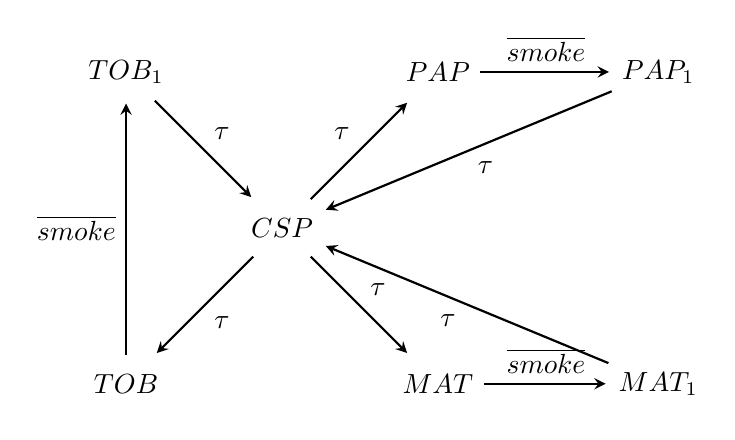
\begin{tikzpicture}[%
 	    ->,
 	    >=stealth,
 	    shorten >=1pt,
 	    node distance=2.8cm,
 	    %on grid,
 	    auto,
 	    state/.append style={minimum size=2em},
 	    thick
 	  ]
 
 
   %\tikzstyle{every state}=[fill=red,draw=none,text=white]
 
 
 	  \node[state] (CSP) {$CSP$};
 	  \node[state] (PAP) [above right of=CSP] {$PAP$};
 	  \node[state] (TOB) [below left of=CSP] {$TOB$};
 	  \node[state] (MAT) [below right of=CSP] {$MAT$};
 	  \node[state] (PAP1) [right of=PAP] {$PAP_{1}$};
    	  \node[state] (TOB1) [above left of=CSP] {$TOB_{1}$};
 	  \node[state] (MAT1) [right of=MAT] {$MAT_{1}$};

 	  \path[->] 
 	      
              (CSP)
		  edge node {$\tau$} (PAP)
		  edge node {$\tau$} (TOB)
		  edge node {$\tau$} (MAT)
 	      (PAP)
		  edge node {$\overline{smoke}$} (PAP1)
 	      (TOB)
		  edge node {$\overline{smoke}$} (TOB1)
 	      (MAT)
		  edge node {$\overline{smoke}$} (MAT1)
 	      (PAP1)
		  edge node {$\tau$} (CSP)
 	      (TOB1)
		  edge node {$\tau$} (CSP)
 	      (MAT1)
		  edge node {$\tau$} (CSP);
          
       \end{tikzpicture}
     \end{center}
  where 
 
 \begin{center}
    \begin{tabular}{l}
      $PAP \stackrel{def}{=} 
	(\nu tob,pap,mat,end)(end().Agent|S_{tob}|S_{mat}|\overline{smoke}.\overline{end}.S_{pap})$
    \\
      $TOB \stackrel{def}{=} 
	(\nu tob,pap,mat,end)(end().Agent|\overline{smoke}.\overline{end}.S_{tob}|S_{mat}|S_{pap})$
    \\
      $MAT \stackrel{def}{=} 
	(\nu tob,pap,mat,end)(end().Agent|S_{tob}|\overline{smoke}.\overline{end}.S_{mat}|S_{pap})$
    \\
      $PAP_{1} \stackrel{def}{=} 
	(\nu tob,pap,mat,end)(end().Agent|S_{tob}|S_{mat}|\overline{end}.S_{pap})$
    \\
      $TOB_{1} \stackrel{def}{=} 
	(\nu tob,pap,mat,end)(end().Agent|\overline{end}.S_{tob}|S_{mat}|S_{pap})$
    \\
      $MAT_{1} \stackrel{def}{=} 
	(\nu tob,pap,mat,end)(end().Agent|S_{tob}|\overline{end}.S_{mat}|S_{pap})$
    \\\\
    \end{tabular}
  \end{center}
\end{example}




\subsection{Low level semantic}
This section contains the definition of an alternative semantic for multi $\pi$. First we define a low level version of the multi $\pi$ calculus, we call this language low multi $\pi$. The low multi $\pi$ is the multi $\pi$ enriched with a marked or intermediate process $*P$:
\begin{center}
   \begin{tabular}{l}
     $P,Q$ ::= $0$ | $\pi.P$ | $P|Q$ | $P+Q$ | $(\nu x) P$ | $A(x_{1}, \cdots, x_{n})$ | $*P$
   \\\\
     $\pi$ ::= $\overline{x}y$ | $x(y)$ | $\underline{\overline{x}y}$ | $\underline{x(y)}$  | $\tau$ 
   \end{tabular}
\end{center}
\begin{definition}
  The low level transition relation is the smallest relation induced by the rules in table \ref{lowleveltransitionrelationearlyIO} in which $P$ stands for a process without mark, $L$ stands for a process with mark and $S$ can stand for both. 
  \begin{table}
    \begin{tabular}{lll}
      \hline\\
	  $\inferrule* [left=\bf{Out}]{
	  }{
	    \overline{x}y.P \stackrel{\overline{x}y}{\longmapsto} P
	  }$
	  &
	  $\inferrule* [left=\bf{EInp}]{
	  }{
	    x(y).P \stackrel{xz}{\longmapsto} P\{z/y\}
	  }$
	  &
	  $\inferrule* [left=\bf{Tau}]{
	  }{
	    \tau.P \stackrel{\tau}{\longmapsto} P
	  }$
      \\\\
      \end{tabular}\\
      \begin{tabular}{ll}
      \\\\
	  $\inferrule* [left=\bf{SOutLow}]{
	  }{
	    \underline{\overline{x}y}.P \stackrel{\overline{x}y}{\longmapsto} * P
	  }$
	  &
	  $\inferrule* [left=\bf{SInpLow}]{
	  }{
	    \underline{x(y)}.P \stackrel{xz}{\longmapsto} * P\{z/y\}
	  }$
      \\\\
      \end{tabular}\\
      \begin{tabular}{lll}
      \\\\
	  $\inferrule* [left=\bf{StarEps}]{
	      S \stackrel{\epsilon}{\longmapsto} S^{'}
	  }{
	      *S \stackrel{\epsilon}{\longmapsto} S^{'}
	  }$
	  &
	  $\inferrule* [left=\bf{StarInp}]{
	      S \stackrel{xy}{\longmapsto} S^{'}
	  }{
	      *S \stackrel{xy}{\longmapsto} S^{'}
	  }$
	  &
	  $\inferrule* [left=\bf{StarOut}]{
	      S \stackrel{\overline{x}y}{\longmapsto} S^{'}
	  }{
	      *S \stackrel{\overline{x}y}{\longmapsto} S^{'}
	  }$
      \\\\
      \end{tabular}\\
      \begin{tabular}{ll}
      \\\\
	  $\inferrule* [left=\bf{Par1R}]{
	      S \stackrel{\gamma}{\longmapsto} S^{'}
% 	    \\ 
% 	      bn(\gamma)\cap fn(Q)=\emptyset
	  }{
	      Q|S \stackrel{\gamma}{\longmapsto} Q|S^{'}
	  }$
	  &
	  $\inferrule* [left=\bf{Par1L}]{
	      S \stackrel{\gamma}{\longmapsto} S^{'}
% 	    \\ 
% 	      bn(\gamma)\cap fn(Q)=\emptyset
	  }{
	      S|Q \stackrel{\gamma}{\longmapsto} S^{'}|Q
	  }$
      \\\\
      \end{tabular}\\
	\begin{tabular}{lll}
	\\\\
	  $\inferrule* [left=\bf{Sum}]{
	    P \stackrel{\gamma}{\longmapsto} S
	  }{
	    P+Q \stackrel{\gamma}{\longmapsto} S
	  }$
	  &
	  $\inferrule* [left=\bf{Cong}]{
	      P\equiv P^{'}
	    \\
	      P^{'} \stackrel{\gamma}{\longmapsto} S
	  }{
	      P \stackrel{\gamma}{\longmapsto} S
	  }$
	  &
	  $\inferrule* [left=\bf{Res}]{
	      S \stackrel{\gamma}{\longmapsto} S^{'}
	    \\
	      y\notin n(\gamma)
	  }{
	    (\nu y) S \stackrel{\gamma}{\longmapsto} (\nu y) S^{'}
	  }$
      \\\\
    \end{tabular}\\
      \begin{tabular}{ll}
      \\\\
	  $\inferrule* [left=\bf{Com1}]{
	      P \stackrel{\overline{x}y}{\longmapsto} P^{'}
	    \\
	      Q \stackrel{xy}{\longmapsto} Q^{'}
	  }{
	    P|Q \stackrel{\tau}{\longmapsto} P^{'}|Q^{'}
	  }$
	  &
       \\\\
	  $\inferrule* [left=\bf{Com2LOut}]{
	      L_{1} \stackrel{\overline{x}y}{\longmapsto} L_{1}^{'}
	    \\
	      L_{2} \stackrel{xy}{\longmapsto} S
	  }{
	    L_{1}|L_{2} \stackrel{\epsilon}{\longmapsto} L_{1}^{'}|S
	  }$
	  &
	  $\inferrule* [left=\bf{Com2ROut}]{
	      L_{1} \stackrel{xy}{\longmapsto} S
	    \\
	      L_{2} \stackrel{\overline{x}y}{\longmapsto} L_{2}^{'}
	  }{
	    L_{1}|L_{2} \stackrel{\epsilon}{\longmapsto} S|L_{2}^{'}
	  }$
       \\\\
	  $\inferrule* [left=\bf{Com2LInp}]{
	      L_{1} \stackrel{\overline{x}y}{\longmapsto} S
	    \\
	      L_{2} \stackrel{xy}{\longmapsto} L_{2}^{'}
	  }{
	    L_{1}|L_{2} \stackrel{\epsilon}{\longmapsto} S|L_{2}^{'}
	  }$
	  &
	  $\inferrule* [left=\bf{Com2RInp}]{
	      L_{1} \stackrel{xy}{\longmapsto} L_{1}^{'}
	    \\
	      L_{2} \stackrel{\overline{x}y}{\longmapsto} S
	  }{
	    L_{1}|L_{2} \stackrel{\epsilon}{\longmapsto} L_{1}^{'}|S
	  }$
       \\\\
	  $\inferrule* [left=\bf{Com3LOut}]{
	      Q \stackrel{\overline{x}y}{\longmapsto} S
	    \\
	      P \stackrel{xy}{\longmapsto} L
	  }{
	    Q|P \stackrel{\epsilon}{\longmapsto} S|L
	  }$
	  &
	  $\inferrule* [left=\bf{Com3ROut}]{
	      P \stackrel{xy}{\longmapsto} L
	    \\
	      Q \stackrel{\overline{x}y}{\longmapsto} S
	  }{
	    P|Q \stackrel{\epsilon}{\longmapsto} L|S
	  }$
       \\\\
	  $\inferrule* [left=\bf{Com3LInp}]{
	      Q \stackrel{xy}{\longmapsto} S
	    \\
	      P \stackrel{\overline{x}y}{\longmapsto} L
	  }{
	    Q|P \stackrel{\epsilon}{\longmapsto} S|L
	  }$
	  &
	  $\inferrule* [left=\bf{Com3RInp}]{
	      P \stackrel{\overline{x}y}{\longmapsto} L
	    \\
	      Q \stackrel{xy}{\longmapsto} S
	  }{
	    P|Q \stackrel{\epsilon}{\longmapsto} L|S
	  }$
	\\\\
	  $\inferrule* [left=\bf{Com4L}]{
	      L_{1} \stackrel{\overline{x}y}{\longmapsto} P
	    \\
	      L_{2} \stackrel{xy}{\longmapsto} Q
	  }{
	    L_{1}|L_{2} \stackrel{\tau}{\longmapsto} P|Q
	  }$
	  &
	  $\inferrule* [left=\bf{Com4R}]{
	      L_{1} \stackrel{xy}{\longmapsto} P
	    \\
	      L_{2} \stackrel{\overline{x}y}{\longmapsto} Q
	  }{
	    L_{1}|L_{2} \stackrel{\tau}{\longmapsto} P|Q
	  }$
	\\\\\hline
	\end{tabular}
    \caption{Low multi $\pi$ early semantic with structural congruence}
    \label{lowleveltransitionrelationearlyIO}
  \end{table}
\end{definition}

% \begin{proposition}
%   Let $\rightarrow$ be the relation defined in table \ref{multiIOearly}, let $P$ and $Q$ be processes and $\alpha$ be an action. Then 
%   \begin{center}
%     \begin{tabular}{lll}
%       $P\xrightarrow{\alpha} Q$
%     &
%       $\Leftrightarrow$
%     &
%       $P\stackrel{\alpha}{\longmapsto} Q$
%     \end{tabular}
%   \end{center}
% \end{proposition}











\begin{proposition}\label{multipiIOloweqright}
  Let $\rightarrow$ be the relation defined in table \ref{multiIOearly}. If $P\xrightarrow{\sigma} Q$ then there exist $L_{1}, \cdots, L_{k}$ and $\gamma_{1}, \cdots, \gamma_{k+1}$ with $k\geq 0$ such that 
  \begin{center}
    \begin{tabular}{lll}
      $P \stackrel{\gamma_{1}}{\longmapsto} L_{1} \stackrel{\gamma_{2}}{\longmapsto} L_{2} \cdots L_{k-1} \stackrel{\gamma_{k}}{\longmapsto} L_{k} \stackrel{\gamma_{k+1}}{\longmapsto} Q$ 
    &
      and
    &
      $\gamma_{1} \cdot \ldots \cdot \gamma_{k+1} = \sigma$  
    \end{tabular}
  \end{center}
  \begin{proof}
    The proof is by induction on the depth of the derivation tree of $P\xrightarrow{\sigma} Q$:
    \begin{description}
      \item[base case]
    \end{description}
	If the depth is one then the rule used have to be one of: $EInp$, $Out$, $Tau$. These rules are also in table \ref{lowleveltransitionrelationearlyIO} so we can derive $P \stackrel{\sigma}{\longmapsto}Q$.
    \begin{description}
      \item[inductive case]
    \end{description}
	If the depth is greater than one then the last rule used in the derivation can be:
	\begin{description}
	  \item[$SOut$]: 
	    the last part of the derivation tree looks like this:
	    \begin{center}
	      $\inferrule* [left=\bf{SOut}]{
		  P_{1} \xrightarrow{\sigma} Q
		\\
		  \sigma \neq \tau
	      }{
		\underline{\overline{x}y}.P_{1} \xrightarrow{\overline{x}y \cdot \sigma} Q
	      }$	      
	    \end{center}
	    for inductive hypothesis there exist $L_{1}, \cdots, L_{k}$ and $\gamma_{1}, \cdots, \gamma_{k+1}$ with $k\geq 0$ such that 
	    \begin{center}
	      \begin{tabular}{lll}
		$P_{1} \stackrel{\gamma_{1}}{\longmapsto} L_{1} \stackrel{\gamma_{2}}{\longmapsto} L_{2} \cdots L_{k-1} \stackrel{\gamma_{k}}{\longmapsto} L_{k} \stackrel{\gamma_{k+1}}{\longmapsto} Q$ 
	      &
		and
	      &
		$\gamma_{1} \cdot \ldots \cdot \gamma_{k+1} = \sigma$
	      \end{tabular}
	    \end{center}
	    then a proof of the conclusion follows from:
	    \begin{center}
	      \begin{tabular}{ll}
		$\inferrule* [left=\bf{SOutLow}]{
 		}{
 		  \underline{\overline{x}y}.P_{1} \stackrel{\overline{x}y}{\longmapsto} *P_{1}
 		}$
	      &
		$\inferrule* [left=\bf{Star}]{
 		  P_{1} \stackrel{\gamma_{1}}{\longmapsto} L_{1}
 		}{
 		  *P_{1} \stackrel{\gamma_{1}}{\longmapsto} L_{1}
 		}$
	      \end{tabular}
	    \end{center}
	  \item[$SInp$]: this case is similar to the previous.
	  \item[$Sum$]: 
	the last part of the derivation tree looks like this:
	\begin{center}
	  $\inferrule* [left=\bf{Sum}]{
	    P_{1} \xrightarrow{\sigma} Q
	  }{
	    P_{1}+P_{2} \xrightarrow{\sigma} Q
	  }$
	\end{center}
	for the inductive hypothesis there exist $L_{1}$, $\cdots$, $L_{k}$ and $\gamma_{1}$, $\cdots$, $\gamma_{k+1}$ with $k\geq 0$ such that 
	\begin{center}
	  \begin{tabular}{lll}
	    $P_{1} \stackrel{\gamma_{1}}{\longmapsto} L_{1} \stackrel{\gamma_{2}}{\longmapsto} L_{2} \cdots L_{k-1} \stackrel{\gamma_{k}}{\longmapsto} L_{k} \stackrel{\gamma_{k+1}}{\longmapsto} Q$ 
	  &
	    and
	  &
	    $\gamma_{1} \cdot \ldots \cdot \gamma_{k+1} =  \sigma$  
	  \end{tabular}
	\end{center}
	A proof of the conclusion is:
	\begin{center}
	  $\inferrule* [left=\bf{Sum}]{
	      P_{1} \stackrel{\gamma_{1}}{\longmapsto} L_{1}
	    }{
	      P_{1}+P_{2} \stackrel{\gamma_{1}}{\longmapsto} L_{1}
	    }
	  $
	\end{center}
      \item[$Cong$]: this case is similar to the previous.
      \item[$Res$]: 
	the last part of the derivation tree looks like this:
	\begin{center}
	  $\inferrule* [left=\bf{Res}]{
	      P_{1}\; \xrightarrow{\sigma}\; Q_{1}
	    \\
	      z\notin n(\sigma)
	  }{
	    (\nu z) P_{1} \;\xrightarrow{\sigma} (\nu z) Q_{1}
	  }$
	\end{center}
	for the inductive hypothesis there exist $L_{1}, \cdots, L_{k}$ and $\gamma_{1}, \cdots, \gamma_{k+1}$ with $k\geq 0$ such that 
	\begin{center}
	  \begin{tabular}{lll}
	    $P_{1} \stackrel{\gamma_{1}}{\longmapsto} L_{1}  \stackrel{\gamma_{2}}{\longmapsto} L_{2} \cdots L_{k-1} \stackrel{\gamma_{k}}{\longmapsto} L_{k} \stackrel{\gamma_{k+1}}{\longmapsto} Q_{1}$ 
	  &
	    and
	  &
	    $\gamma_{1} \cdot \ldots \cdot \gamma_{k+1} =  \sigma$
	  \end{tabular}
	\end{center}
	We can apply the rule $Res$ to each of the previous transitions because 
	\begin{center}
	  $z\notin n(\sigma)$ implies $z\notin n(\gamma_{i})$ for each $i$
	\end{center}
	and then get a proof of the conclusion:
	\begin{center}
	  $(\nu z)P_{1} \stackrel{\gamma_{1}}{\longmapsto} (\nu z)L_{1}  \stackrel{\gamma_{2}}{\longmapsto} (\nu z)L_{2} \cdots (\nu z)L_{k-1} \stackrel{\gamma_{k}}{\longmapsto} (\nu z)L_{k} \stackrel{\gamma_{k+1}}{\longmapsto} (\nu z)Q_{1}$
	\end{center}
      \item[$Par$]: this case is similar to the previous.
      \item[$ECom$]: 
	the last part of the derivation tree looks like this:
	\begin{center}
	  $\inferrule* [left=\bf{ECom}]{
	      P_{1} \xrightarrow{\sigma_{1}} P_{1}^{'}
	    \\
	      Q_{1} \xrightarrow{\sigma_{2}} Q_{1}^{'}
	    \\
	      ESync(\sigma_{1}, \sigma_{2}, \sigma_{3})
	  }{
	    P_{1}|Q_{1} \xrightarrow{\sigma_{3}} P_{1}^{'}|Q_{1}^{'}
	  }$
	\end{center}
	for inductive hypothesis there exist $L_{1}, \cdots, L_{k}$ and $\gamma_{1}, \cdots, \gamma_{k+1}$ with $k\geq 0$ such that 
	\begin{center}
	  \begin{tabular}{lll}
	    $P_{1} \stackrel{\gamma_{1}}{\longmapsto} L_{1}  \stackrel{\gamma_{2}}{\longmapsto} L_{2} \cdots L_{k-1} \stackrel{\gamma_{k}}{\longmapsto} L_{k} \stackrel{\gamma_{k+1}}{\longmapsto} P_{1}^{'}$ 
	  &
	    and
	  &
	    $\gamma_{1} \cdot \ldots \cdot \gamma_{k+1} = \sigma_{1}$
	  \end{tabular}
	\end{center}
	and there exist $R_{1}, \cdots, R_{h}$ and $\delta_{1}, \cdots, \delta_{h+1}$ with $h\geq 0$ such that 
	\begin{center}
	  \begin{tabular}{lll}
	    $Q_{1} \stackrel{\delta_{1}}{\longmapsto} R_{1}  \stackrel{\delta_{2}}{\longmapsto} R_{2} \cdots R_{h-1} \stackrel{\delta_{h}}{\longmapsto} R_{h} \stackrel{\delta_{h+1}}{\longmapsto} Q_{1}^{'}$ 
	  &
	    and
	  &
	    $\delta_{1} \cdot \ldots \cdot \delta_{h+1} = \sigma_{2}$
	  \end{tabular}
	\end{center}
	We proceed by cases on the derivation of $ESync(\sigma_{1}, \sigma_{2}, \sigma_{3})$. We show just some cases because the others are similar.
	\begin{description}
	  \item[$S1L$] 
	    Suppose that $\delta_{1}$ is $\overline{x}y$(the other cases are similar), so the other $\delta$s are $\epsilon$ or $\tau$. We can have three different cases now each : 
	    \begin{description}
	      \item[$\gamma_{1}=xy$]:
		The other $\gamma$s are $\epsilon$ or $\tau$. A proof of the conclusion is:
		  \begin{center}
		    $P_{1}|Q_{1} 
		      \stackrel{\epsilon}{\longmapsto} 
			L_{1}|R_{1}
		      \stackrel{\epsilon}{\longmapsto} 
			L_{2}|R_{1}
		      \cdots
		      \stackrel{\epsilon}{\longmapsto} 
			P_{1}^{'}|R_{1}
		      \stackrel{\epsilon}{\longmapsto} 
			P_{1}^{'}|R_{2}
		      \cdots
		      \stackrel{\epsilon}{\longmapsto} 
			P_{1}^{'}|Q_{1}^{'}$
		  \end{center}
		we derive the first transition with rule $Com3ROut$, whether for the other transition we use the rules $Par1L$, $Par1R$, $Par3L$ or $Par3R$.
	      \item[$\gamma_{i}=xy$]:
		A proof of the conclusion is:
		  \begin{center}
		    $P_{1}|Q_{1} \stackrel{\epsilon}{\longmapsto} L_{1}|Q_{1} 
		      \cdots
 			      \stackrel{\epsilon}{\longmapsto} L_{i-1}|Q_{1} 
 			      \stackrel{\tau}{\longmapsto} L_{i}|R_{1}
 			      \stackrel{\epsilon}{\longmapsto} L_{i+1}|R_{1}
		      \cdots 
 			      \stackrel{\epsilon}{\longmapsto} P_{1}^{'}|R_{1}
 			      \stackrel{\epsilon}{\longmapsto} P_{1}^{'}|R_{2}
		      \cdots 
 			      \stackrel{\epsilon}{\longmapsto} P_{1}^{'}|Q_{1}^{'}$
		  \end{center}
		we derive the transaction $ L_{i-1}|Q_{1} \stackrel{\tau}{\longmapsto} L_{i}|R_{1}$ with rule $Com5L$, whether for the other transactions we use some rule for parallel.
	      \item[$\gamma_{k+1}=xy$] similar.
	    \end{description}
	  \item[$S2R$]: 
	    We suppose that $\delta_{1}=xy$ and so other $\delta$s are $\epsilon$ or $\tau$, the other cases are similar. We can have two different cases now depending on where the first $\overline{x}y$ is:
	      \begin{description}
		\item[$\gamma_{1}=\overline{x}y$]:
		  A proof of the conclusion is:
		  \begin{center}
		    $P_{1}|Q_{1} \stackrel{\tau}{\longmapsto} L_{1}|R_{1}
 			      \stackrel{\gamma_{2}}{\longmapsto} L_{2}|R_{1}
			\cdots
 			      \stackrel{\gamma_{k+1}}{\longmapsto} P_{1}^{'}|R_{1}
			      \stackrel{\delta_{2}}{\longmapsto} P_{1}^{'}|R_{2}
			\cdots
			      \stackrel{\delta_{h+1}}{\longmapsto} P_{1}^{'}|Q_{1}^{'}$
		  \end{center}
		  we derive the first transition with rule $Com3L$, whether for the other transactions we use some rule for parallel. Since $\gamma_{1} \cdot \ldots \cdot \gamma_{k+1} = \overline{x}y \cdot \sigma$ and $\gamma_{1}=\overline{x}y$ then $\tau \cdot \gamma_{2}\cdot \ldots \cdot \gamma_{k+1}\cdot \epsilon \cdot \ldots \epsilon \cdot \tau=\sigma$
		\item[$\gamma_{i}=\overline{x}y$]:
		  A proof of the conclusion is:
		  \begin{center}
		    $P_{1}|Q_{1} \stackrel{\epsilon}{\longmapsto} L_{1}|Q_{1} 
			\cdots
 			      \stackrel{\epsilon}{\longmapsto} L_{i-1}|Q_{1} 
 			      \stackrel{\tau}{\longmapsto} L_{i}|R_{1}
 			      \stackrel{\gamma_{i+1}}{\longmapsto} L_{i+1}|R_{1}
			\cdots 
 			      \stackrel{\gamma_{k}}{\longmapsto} P_{1}^{'}|R_{1}
 			      \stackrel{\delta_{2}}{\longmapsto} P_{1}^{'}|R_{2}
			\cdots 
 			      \stackrel{\delta_{h+1}}{\longmapsto} P_{1}^{'}|Q_{1}^{'}$	  
		  \end{center}
		  we derive the transition $L_{i-1}|Q_{1} \stackrel{\tau}{\longmapsto} L_{i}|Q_{1}^{'}$ with rule $Com2L$, whether for the other transactions of the premises we use the rule $Par1L$.
		\item[$\gamma_{k+1}=\overline{x}y$]: cannot happen because $\sigma$ is not empty.
	      \end{description}
	    \item[$S4R$]
	      We have three cases: $|\sigma_{1}|=|\sigma_{2}|$, $|\sigma_{1}|>|\sigma_{2}|$ or $|\sigma_{2}|>|\sigma_{1}|$. In the first case $|\sigma_{3}|$ must be $\tau$ and we can build a chain of transition as in the previous cases. In the second case there is a prefix of $\sigma_{1}$ which synchronize with $\sigma_{2}$ and $\sigma_{3}$ is the rest of $\sigma_{1}$, in this case we can also build a chain of transition as in the previous cases. The third case is symmetric to the second.
	  \end{description}
    \end{description}
  \end{proof}
\end{proposition}


The converse of lemma \ref{multipiIOloweqright} does not hold because the low semantic allow to express interleaving behaviour. But there is the following weaker result:
\begin{proposition}
  Let $\rightarrow$ be the relation defined in table \ref{multiIOearly}, let $\alpha$ be an action and $P,Q$ be processes. If $P \stackrel{\alpha}{\longmapsto} Q$ then $P\xrightarrow{\alpha} Q$.
  \begin{proof}
    The proof is an easy induction on the proof tree of $P \stackrel{\alpha}{\longmapsto} Q$.
  \end{proof}
\end{proposition}














